%!TEX root = main.tex

% Introduction for negFE
\section{Introduction}
Information reconciliation and privacy amplification are the two
fundamental tasks for key derivation from noisy sources.  Roughly
speaking, information reconciliation takes two correlated
distributions $w$ and $w'$ and maps them to the same value while
minimizing what is leaked about that value.  Privacy amplification
converts the uncertainty in this mapped value to a uniform value
suitable for cryptography.  Applications areas include quantum key
agreement, biometrics, and physically uncloneable
functions~\cite{bennett1988privacy,dodis2008fuzzy}.

We focus on non-interactive versions of these problems~\cite{dodis2008fuzzy} as defined by secure sketches, which perform information-recon\-ciliation, and fuzzy extractors, which perform both information-recon\-ciliation and privacy amplification. A Secure Sketch consists of a pair of algorithms $(\sketch, \rec)$ where:
\begin{enumerate}
\item $\sketch(w) = ss$ should reveal as little information as possible about $w$; and
\item $\sketch(w) =ss$ should allow one to reconstruct $w$ from a nearby $w'$. That is, it should be the case that for all nearby $w', \rec(w', ss) = w$.  In the above, ``nearby'' is $w'$ such that $\dis(w,w')\le t$ for  distance metric $\dis$ and distance $t$.
\end{enumerate}
These two properties are in tension because allowing recovery of $w$ requires information about $w$.  The most natural (inefficient) construction is for $ss$ to be a pairwise independent~\cite{carter1977universal} hash $h$ of $w$~\cite{skoric2009efficient,fuller2016fuzzy,woodage2017new,fuller2020fuzzy}. The hash $h$ should be long enough so that $\{w | h(w) = y \wedge w' s.t.\,\dis(w, w')\le t\} =1$ and short enough so $\{w| h(w) = y\}$ is large. Efficient constructions are also known based on error-correcting codes.  In fact, upper bounds on the unpredictability of $w | ss$ are related to the size of the best error-correcting codes~\cite{dodis2008fuzzy,fuller2020computational}. 
Given a good information reconciliation, one can achieve privacy amplification using an average-case randomness extractor~\cite{nisan1993randomness} to convert $w$ into a uniform value.

  Fuzzy extractors perform both information reconciliation and privacy amplification.  They consist of a pair $(\gen, \rep$).  Intuitively, $\gen$ converts a value $w$ into a uniform value, denoted as $r$ and $\rep$ reproduces that value for any nearby $w'$.  Notationally, $(r, p)\leftarrow \gen(w)$ should be indistinguishable from $(u, p)$ where $u$ is a truly random value.  On the correctness side, it should be the case that for all $w'$ such that $\dis(w, w')\le t$ then $\rep(w', p) =r$.  
  Both $\sketch$ and $\gen$ are allowed to have private internal randomness.  
  
  
Since noisy sources come from the physical world, an important goal
  is to be able to support as many distributions $W$ as possible. This goal is the focus of this work. 
  Throughout the Introduction, we use the notation of fuzzy extractors
  and note when there are material differences for secure sketches.
  Fuller, Reyzin, and Smith~\cite{fuller2016fuzzy,fuller2020fuzzy}
  identified the notion of fuzzy min-entropy $\Hfuzz(W)$ which
  measures the adversary's success when given oracle access to
  $\rep(\cdot, p)$ but is unable to learn anything from the value $p$.
Fuzzy min-entropy quantifies the weight of the heaviest ball
  in the probability mass function of $W$.  That is,
\[
\Hfuzz(W):= -\log{\max_{w'} \sum_{w } \Pr[W=w | \dis(w, w')\le t]}.
\]Ideally, one would build a single fuzzy extractor that works for the family of all distributions $\Wallfuzz = \{ W | \Hfuzz(W) = \omega(\log \lambda)\}$ for some security parameter $\lambda$.  We call such a fuzzy extractor \emph{universal} as it simultaneously works for any secureable distribution $W$. 
If one desires computational security, a universal fuzzy extractor is achievable using general obfuscation~\cite{BarakBCKPS13,BitanskyCKP14,bitansky2017virtual} or under specific number-theoretic assumptions~\cite{galbraith2019obfuscated}. 


The situation for information-theoretic security is more
complicated.\footnote{Fuzzy extractors were first designed as an
  information-theoretic primitive because of strong connections to
  randomness extraction and coding theory.  An important application is in quantum key agreement which does not allow computational assumptions.  Many computational
  constructions use an information-theoretic secure
  sketch~\cite{wen2018robustly,wen2019generic}.  (Exceptions exist
  such as the universal constructions listed above and constructions
  for distributions with additional
  properties~\cite{apon2017efficient,alamelou2018pseudoentropic,fuller2020computational,canetti2021reusable}.)
}  Fuller, Reyzin, and Smith~\cite{fuller2020fuzzy} showed that it is
impossible to build a universal fuzzy extractor with
information-theoretic security.  More precisely, they constructed a
family of distributions $\mathcal{W}'$ and showed that any
fuzzy extractor $(\gen, \rep)$ must be insecure for an average member
of $\mathcal{W}'$. Let $z$ be a string that indexes the family $\mathcal{W}'$. We use $Z$ to describe a uniformly chosen index for
the family $\mathcal{W'}$.  We use the notation $z\leftarrow Z$ to indicate this choice. We use the notation $W_Z$ to indicate sampling $W$ uniformly from $\mathcal{W}$ with $Z$ being a random variable that describes the choice of $W\in\mathcal{W}$. For all $z$, the goal is to build a good fuzzy extractor for $W_z$.  The impossibility result shows a family $\mathcal{W}'$ where any $(\gen, \rep)$ is insecure for an average $z$ chosen according to $Z$.  The model tells the adversary the outcome $Z=z$ but not the
individual point $w\leftarrow W_z$ that is input to $\gen$.

On the positive side, multiple works~\cite{hayashi2014secret,hayashi2016secret,fuller2016fuzzy,woodage2017new,tyagi2017universal,TVW18,LA18,fuller2019continuous,fuller2020fuzzy} presented a construction that works for each $W_z\in \Wallfuzz$.  This is called the \emph{distribution-sensitive} setting as $\gen$ also knows the entire probability mass function described by $z$, denoted as $\gen_{z}, \rec_{z}$.  All constructions in this line are computationally inefficient; for an input point $w$ they look up the probability that $\Pr[W_z=w]$ and the probability of points $w'$ where $\dis(w, w')\le t$.  
%Thus, there is a large gap between the state of affairs with computational and information-theoretic security.  With computational security, universal fuzzy extractors are possible.  With information-theoretic security universal fuzzy extractors are impossible.  Furthermore, known distribution-sensitive fuzzy extractors require information about $W$ proportional to its description.  

We show this inefficiency is unavoidable:
\begin{displayquote}
\textbf{Any distribution-sensitive information-theoretic fuzzy extractor requires an exponential amount of information about the distribution $W_z$.} 
\end{displayquote} 
Our results are for the Hamming metric over $\zo^n$. Below we present the two informal theorems for fuzzy extractors (see Theorem~\ref{thm:main theorem}) and secure sketches (see Theorem~\ref{thm:main theorem ss}) respectively.  For a value $p\in [0,1]$ let $h_2$ be the binary entropy of $p$. 
Both secure sketches and fuzzy extractor are frequently parameterized by an error parameter $\delta$ which controls the maximum probability they get the wrong value.  We consider $\delta=0$ for the fuzzy extractor setting and $\delta>0$ for the secure sketch setting. 

\begin{theorem}[Informal Theorem~\ref{thm:main theorem}]
Consider $\zo^n$ and $t< n/2$ be a distance parameter.  Let $\mathcal{W}_\gamma=\{W | \Hfuzz(W) = \gamma\}$.  Let $c>0$ be a constant and suppose that \[
\gamma \le n\cdot\min\left\{(1-h_2(t/n)) +o(1), \frac{1-\Theta(c)-h_2(1/2-t/n)}{3}\right\}.
\]
 For a quarter of $W \in \mathcal{W}_\gamma$ there is no fuzzy extractor that simultaneously has 
 \begin{enumerate}
 \itemsep0em
 \item no error,
 \item is of size at most $2^{\gamma+cn}$, and 
 \item extracts keys of length $\omega(\log n)$ that are within statistical distance $1/3-\ngl(n)$ to a uniform key.
 \end{enumerate}
\end{theorem}


\begin{theorem}[Informal Theorem~\ref{thm:main theorem ss}]
Consider $\zo^n$ and $t< n/2$ be a distance parameter.  Let $\mathcal{W}_\gamma=\{W | \Hfuzz(W) = \gamma\}$.  Let $\delta<1/4$ be the error of the secure sketch, let $c>0$ be a constant and suppose that \[
\gamma \le n\cdot\min\left\{(1-h_2(t/n)) +o(1), c_\delta h_2(t/n)-\Theta(c)\right\}.
\]
where $1/3\le  c_\delta \le 2/3$ and depends on $h_2(\delta)$. 
 For $2^{-5}$ fraction of $W \in \mathcal{W}_\gamma$ there is no secure sketch of
size of at most $2^{\gamma+cn}$ that
 retains unpredictability of $w|ss$ of at  least $5$.
\end{theorem}

\begin{figure}[t]
\centering
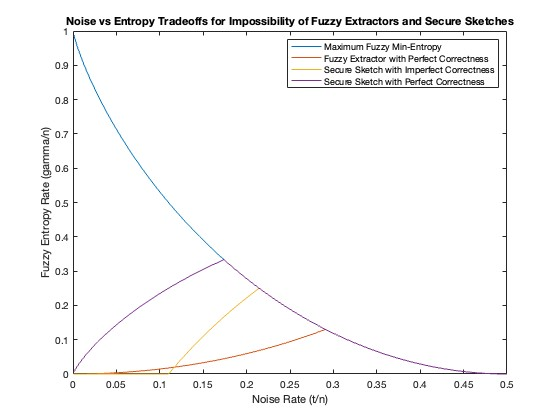
\includegraphics[width=.9\textwidth]{EntropyvsError.jpg}
\caption{The region of error rate $t/n$ ($x$-axis) and fuzzy entropy rate $\gamma/n$ (y-axis) pairs for which the two negative results apply.  The six curves are maximum fuzzy min-entropy $\gamma/n = (1-h_2(t/n))$, Theorem~\ref{thm:main theorem}, Theorem~\ref{thm:main theorem ss} with $\delta=.25$,  Theorem~\ref{thm:main theorem ss} with $\delta =0$, \cite[Theorem 5.1]{fuller2020fuzzy} and \cite[Theorem 7.2]{fuller2020fuzzy}. The parameter $\delta$ is how frequently the secure sketch is allowed to be incorrect.  We consider fuzzy extractors with perfect correctness where $\delta=0$.}
\label{fig:param regime}
\end{figure}
The \emph{size} of the fuzzy extractor (resp. secure sketch) refers to the amount of information the algorithm has about $z$, it is not a restriction on the running time of the algorithm, our results hold for unbounded time algorithms. 
 The relevant parameter regimes of impossibility are shown in Figure~\ref{fig:param regime}.  The two most important parameters are the noise rate $t/n$ and the fuzzy entropy rate $\gamma/n$. The area under the curves represents parameters where the construction is impossible for the fraction of distributions in the informal theorems unless one has algorithms of $2^{\Theta(n)}$ size.
In spirit, our result rules out constructions that do not have a full description of the probability mass function written in their description.  

Our results use only first and second-moment bounds.    \textbf{Our theorems are crucial for the future of information-theoretic fuzzy extractors and secure sketches.  To prove security for an efficient construction one must either restrict to sources with high fuzzy min-entropy or use properties of a noisy source beyond fuzzy min-entropy.}  %Most deployed constructions of fuzzy extractors use an information-theoretic information-reconciliation component and are thus subject to our results. 


%\paragraph{Fuzzy extractors are computational objects} The other
%natural explanation of the result is that non-interactive information
%reconciliation should be considered a computational object. This is
%our preferred interpretation since one can build universal (and
%efficient) fuzzy extractors if computational security suffices.  We
%note that the only known constructions assume either general
%obfuscation~\cite{BarakBCKPS13,BitanskyCKP14,bitansky2017virtual} or
%specific number-theoretic assumptions that are not well
%studied~\cite{galbraith2019obfuscated}. Thus, an important direction
%of research is to understand the required assumptions to build
%efficient, universal fuzzy extractors with computational security.


\subsection{Proof Techniques}
Our results are information-theoretic. We
consider a family of distributions $\mathcal{W} = \{ W_z \}$ indexed by a string $z$.  We let $\mathcal{Z}$ denote the set of possible $z$ and let $Z$
denote the uniform distribution over $\mathcal{Z}$.   
Lastly, we use $w\leftarrow W_z$ to
denote sampling a point from the distribution indexed by $z$.  We show the
impossibility of two types of fuzzy extractors:
\begin{description}
\item[Def.~\ref{def:fe distributional}] (Universal) Fuzzy extractors with distributional advice.  This is a triplet of algorithms $(\advice, \gen, \rep)$ designed to work for all $W_z \in \mathcal{W}_\gamma$ for a fixed error tolerance $t$.  The fuzzy extractor is given information about $z$ through a function $\advice = \advice(z)$ which is input to both $\gen$ and $\rep$. The value of $\advice$ \emph{specializes} $(\gen, \rep)$ to the distribution described by $z$. 

Define $w\leftarrow W_z$ and $(r, p) \leftarrow \gen(w, \advice)$, it should be true that 
\[
(r, p, z) \approx (u, p, z).
\] 
where $u$ is uniformly and independently sampled.  Since $\advice(\cdot)$ is a function, $\advice$ is available to the adversary. 
\item[Def.~\ref{def:fe}] Fuzzy extractors for a specific distribution $W_z \in \mathcal{W}$ that are required to have a bounded size description of $(\gen, \rep)$.
\end{description}

We show impossibility of building a fuzzy extractor with distributional advice of length $\ell$ for $\mathcal{W}$ implies impossibility of building a space bounded fuzzy extractor for length $\ell$ for a constant fraction of $\mathcal{W}$ (Lemma~\ref{lem:distributional advice suffices}). 
The core of our negative results is to show the impossibility of building fuzzy extractors with distributional advice.   

We review Fuller, Reyzin, and Smith's~\cite{fuller2020fuzzy} impossibility result.
%\paragraph{Review of Fuller, Reyzin, and Smith~\cite{fuller2020fuzzy}}
Fuzzy extractor correctness says that for $(r, p)\leftarrow \gen(w)$ for all $w'$ close to $w$ the correct key is reproduced, i.e., $\rep(w', p)=r$.  As such, for each value of $p$, one can partition the input space $\zo^n$ by what value of $r$ the point  $v\in \zo^n$ produces.  Values $v$ that could have produced  $r$ will be at least distance $t$ from the boundary of this partition, we call the set of such $v$, $\viable_{r,p}$.  $\viable_{r,p}$ can be bounded geometrically using the isoperimetric inequality~\cite{harper1966optimal}.  This bound applies for any distribution over the inputs $w$.

Consider the following simple distinguisher for a triple $r, p, z$.  One computes the key partition described above and the set $\viable_{r,p}$. If $\viable_{r,p} \cap W_z  = \emptyset$ output the key is random, otherwise output key is real. 
The core of Fuller, Reyzin, and Smith's impossibility was to build a family $\mathcal{W}^{FRS}$ with three properties:
\begin{enumerate}
\item The distribution was $2$-universal~\cite{carter1977universal}, so the remainder of the distribution was unknown conditioned on the input $w$. 
\item Distributions $W_z \in \mathcal{W}^{FRS}$ shared few points and had fuzzy min-entropy.
\end{enumerate}
These three properties meant that for any partition $p$ created after seeing $w$ for most distributions $W_z$ where $\Pr[W_z=w]>0$ have few parts with nonempty interiors. Thus, the above distinguisher works.

The family is as follows: let $\mathbf{C}$ be a linear error-correcting code with distance $t$, let $\mathbf{H}$ be its syndrome, let $c$ be a coset.  Then each $z = (\mathbf{H}, c)$ and a distribution $W_{z=(\mathbf{H}, c)}$ is the uniform distribution over  the set of all points $\{w \mid \mathbf{H} w = c\}$.

\paragraph{Moving to the distributional advice setting}
To set notation for the distributional advice game, we consider the following game for a tuple of algorithms $(\advice, \gen, \rep)$:
\begin{enumerate}
\itemsep0em
\item A uniform sample $z\leftarrow Z$ which picks $W_z\in \mathcal{W}$. 
\item A bounded length $\advice = \advice(z)$ is computed.
\item Sample $w\leftarrow W_z$.
\item The algorithm computes $(r, p)\leftarrow \gen(w, \advice)$.
\item The adversary is given either $(r, p, z)$ or $(u, p, z)$ for a uniform $u$. 
\end{enumerate}

In \cite{fuller2020fuzzy}, the only information that $\gen$ has about $z$ was the input point $w$.  In our setting, $\gen$ gets $\advice$.  Fuller, Reyzin, and Smith's family had a short description so $\advice$ allows $\gen$ to align $\viable$ with points in $W_z$.  Thus, extending the result requires a long description that can't be compressed.  We consider the natural candidate: the set $\mathcal{W}_\gamma$ of all distributions with fuzzy min-entropy at least $\gamma$. 

We use the notation $\wnk = \{W | W\text{ has support size }2^k\}$.  For a positive integer $\gamma$, If one considers $k = \gamma +cn$ for some $c>0$ there are few distributions $W_z\in\mathcal{W}_{n,k}$ where $\Hfuzz(W)<\gamma$.  As long as $|\advice|$ is shorter than $2^k$, most points in the support of $W_z$ are unpredictable conditioned on $\advice$.

The techniques for the secure sketch setting are similar, however, there are stronger geometric bounds on the number of viable points because secure sketches imply Shannon error correcting codes~\cite{dodis2008fuzzy,fuller2020computational}.  Our result considers a secure sketch that retains smooth min-entropy instead of min-entropy.  This is so we can use $\mathcal{W}_{n,k}$ throughout the proof and ``smooth'' to a family where every distribution has fuzzy min-entropy $\gamma$.  Our final result also applies to secure sketches that retain non-smooth conditional min-entropy.

Importantly, both results operate generically in the size of the maximum number of viable points for the relevant primitive.  Such bounds have been well established in the literature due to their connections with coding theory.  This means if one can provide a new bound on fuzzy extractor or secure sketch quality this can be directly used in our results. 


\paragraph{Discussion}
As noted above, our proofs  have strong implications for the future of fuzzy extractors, new designs or analyses are necessary.  Our results may give some theoretical backing to why designs of biometric cryptosystems with high security have been difficult to achieve (see discussion in~\cite{simhadri2019cryptographic}).

Our fuzzy extractor result requires that $|r| = \omega(\log n)$.  This is in contrast to Fuller, Reyzin, and Smith~\cite{fuller2020fuzzy} who showed an impossibility for a key length of $3$.\footnote{Our result for secure sketches requires them to retain at least $5$ bits of min-entropy about the input in comparison with \cite{fuller2020computational} which required the sketch to maintain $3$ bits of entropy.} This change comes because $\advice$ can supply a lot of information about a small number of points in $W_z$, allowing $\gen$ to ensure that some $\viable_{r,p}$ are nonempty. Furthermore, all bounds are weaker than those of Fuller, Reyzin, and Smith.  The core of the difference is that since $\mathcal{W}^{FRS}$ the adversary received entirely new information by the leftover hash lemma~\cite{haastad1993construction,barak2011leftover}. In our setting, we argue about the expected number of points in the support of $W_z$ that are included in the $\viable$ region. 

Our secure sketch result also considers an object that retains smooth conditional min-entropy~\cite{renner2005simple}.  %Smooth conditional min-entropy means that one is statistically close to a distribution with min-entropy.  Setting the closeness parameter to $0$ gives traditional conditional min-entropy.  This is so we can conduct the argument using $U_{n,k}$ and ``smooth'' to the family where all distributions have fuzzy min-entropy. 
Smooth conditional min-entropy is the necessary and sufficient condition for privacy amplification using a randomness extractor. 


\paragraph{Organization} The rest of this work is organized as follows, Section~\ref{sec:prelim} covers preliminaries including the relevant definitions of fuzzy extractors and secure sketches.  Section~\ref{sec:fe} presents the negative result for fuzzy extractors including a proof outline, and Section~\ref{sec:ss} presents the negative result for secure sketches.


%%% Local Variables:
%%% mode: latex
%%% TeX-master: "main"
%%% End:
